\documentclass[10pt,journal]{IEEEtran}


\usepackage{amsfonts}
\usepackage{amsmath}
\usepackage{algorithm}
\usepackage{algorithmic}
\usepackage{amssymb}
\usepackage{graphicx}
\usepackage{cite}
\usepackage{subfigure}
\usepackage{float}
\usepackage{color}


\begin{document}


\title{Reverse Engineering Algorithmic Mechanism Behind WeChat Red Envelope}

\author{\IEEEauthorblockN{Shan Zhang}\\
\IEEEauthorblockA{School of Information Science and Technology\\
  ShanghaiTech University}} 
\maketitle

\begin{abstract}
Please state your abstract here.  
\end{abstract}


\section{Introduction}

Please state the background of your problems. \\

The main results and contributions of this report are summarized as follows:
\begin{itemize}
  \item \textbf{Modeling.  }
  \item \textbf{Simulation Verification.}
  \item \textbf{Theoretical Analysis}.    
\end{itemize}


\section{Model and Algorithms}

Please present your model and algorithms here. 



\section{Simulation Results}

Please present your simulation results. 

%%%%%%%%%%%%%%%%%%%%%%%%%%%%%%%%%%%%%%%%%%%%
 \begin{figure}[!ht]
    \centering
    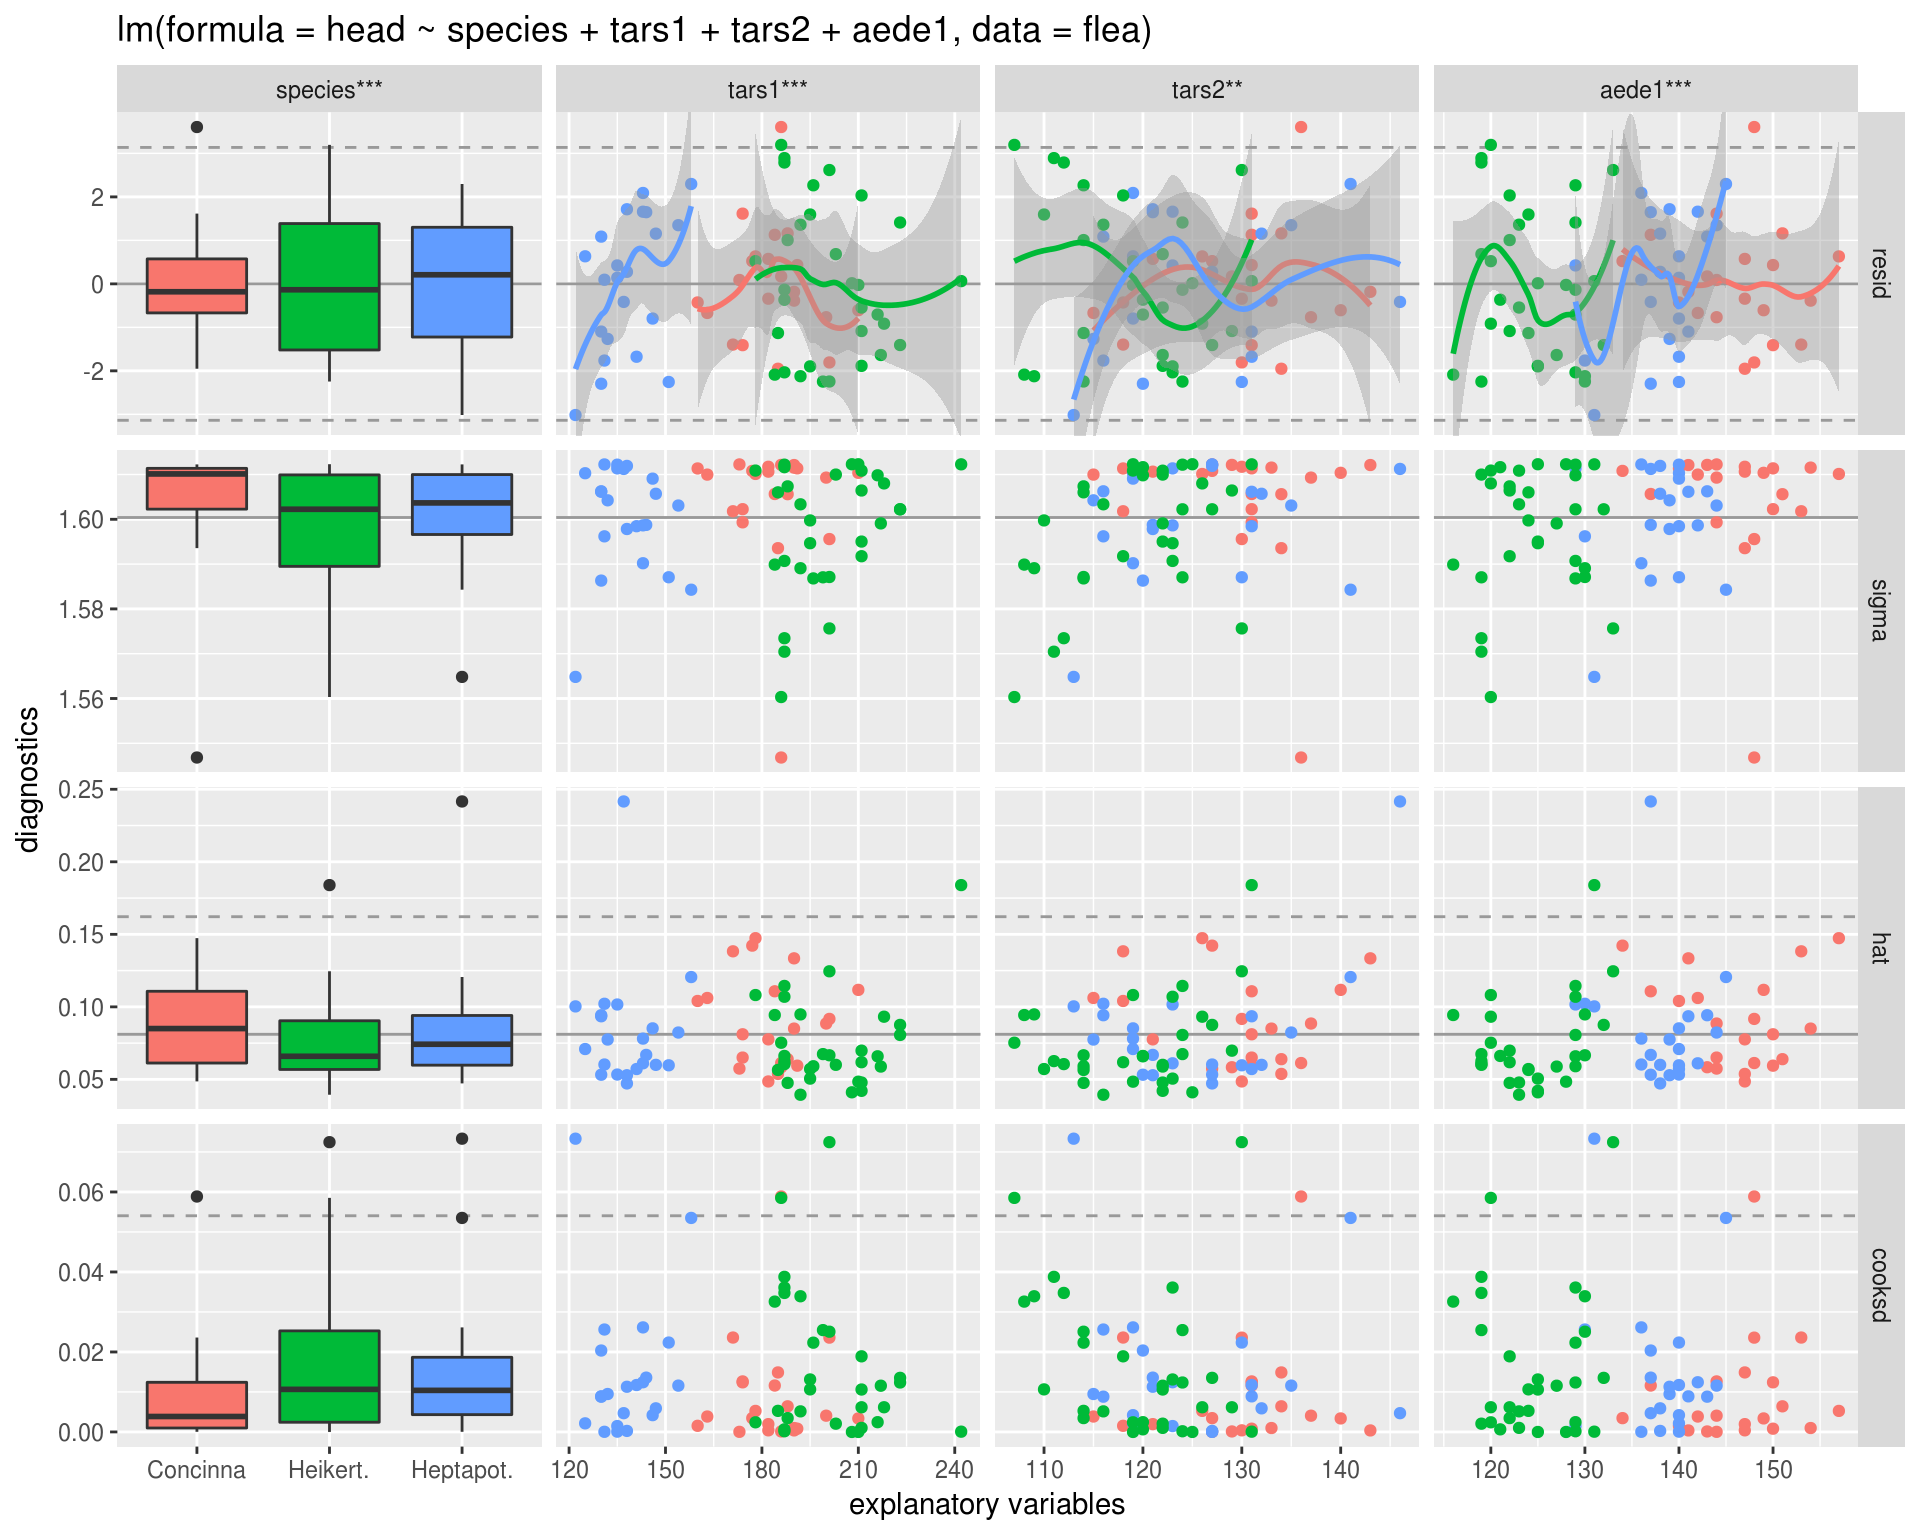
\includegraphics[width=0.9\columnwidth]{Fig/data1.png}
    \caption{Example 1 for Data visualization}
 \end{figure}
%%%%%%%%%%%%%%%%%%%%%%%%%%%%%%%%%%%%%%%%%%%%

%%%%%%%%%%%%%%%%%%%%%%%%%%%%%%%%%%%%%%%%%%%%
 \begin{figure}
    \centering
    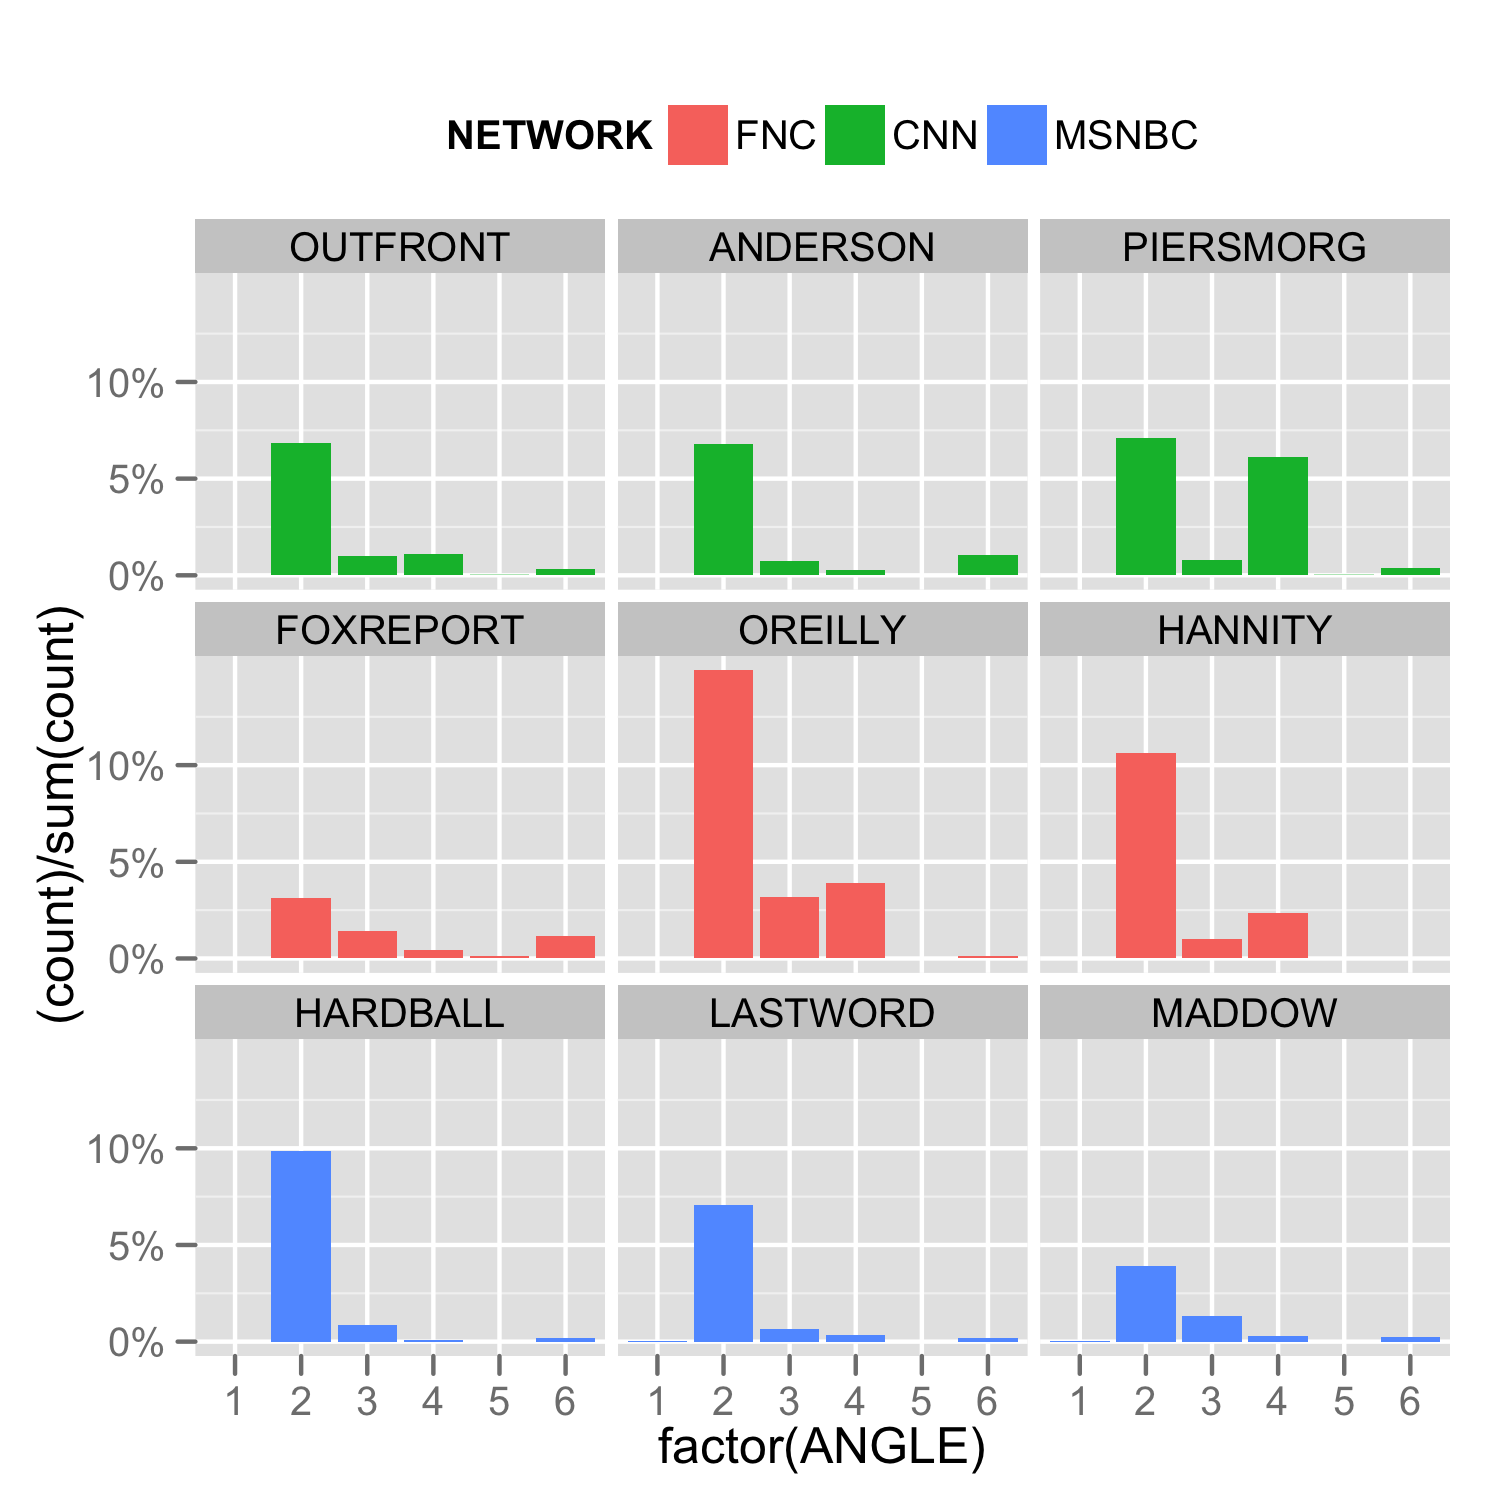
\includegraphics[width=0.9\columnwidth]{Fig/data2.png}
    \caption{Example 2 for Data visualization}
 \end{figure}
%%%%%%%%%%%%%%%%%%%%%%%%%%%%%%%%%%%%%%%%%%%%

%%%%%%%%%%%%%%%%%%%%%%%%%%%%%%%%%%%%%%%%%%%%
 \begin{figure}
    \centering
    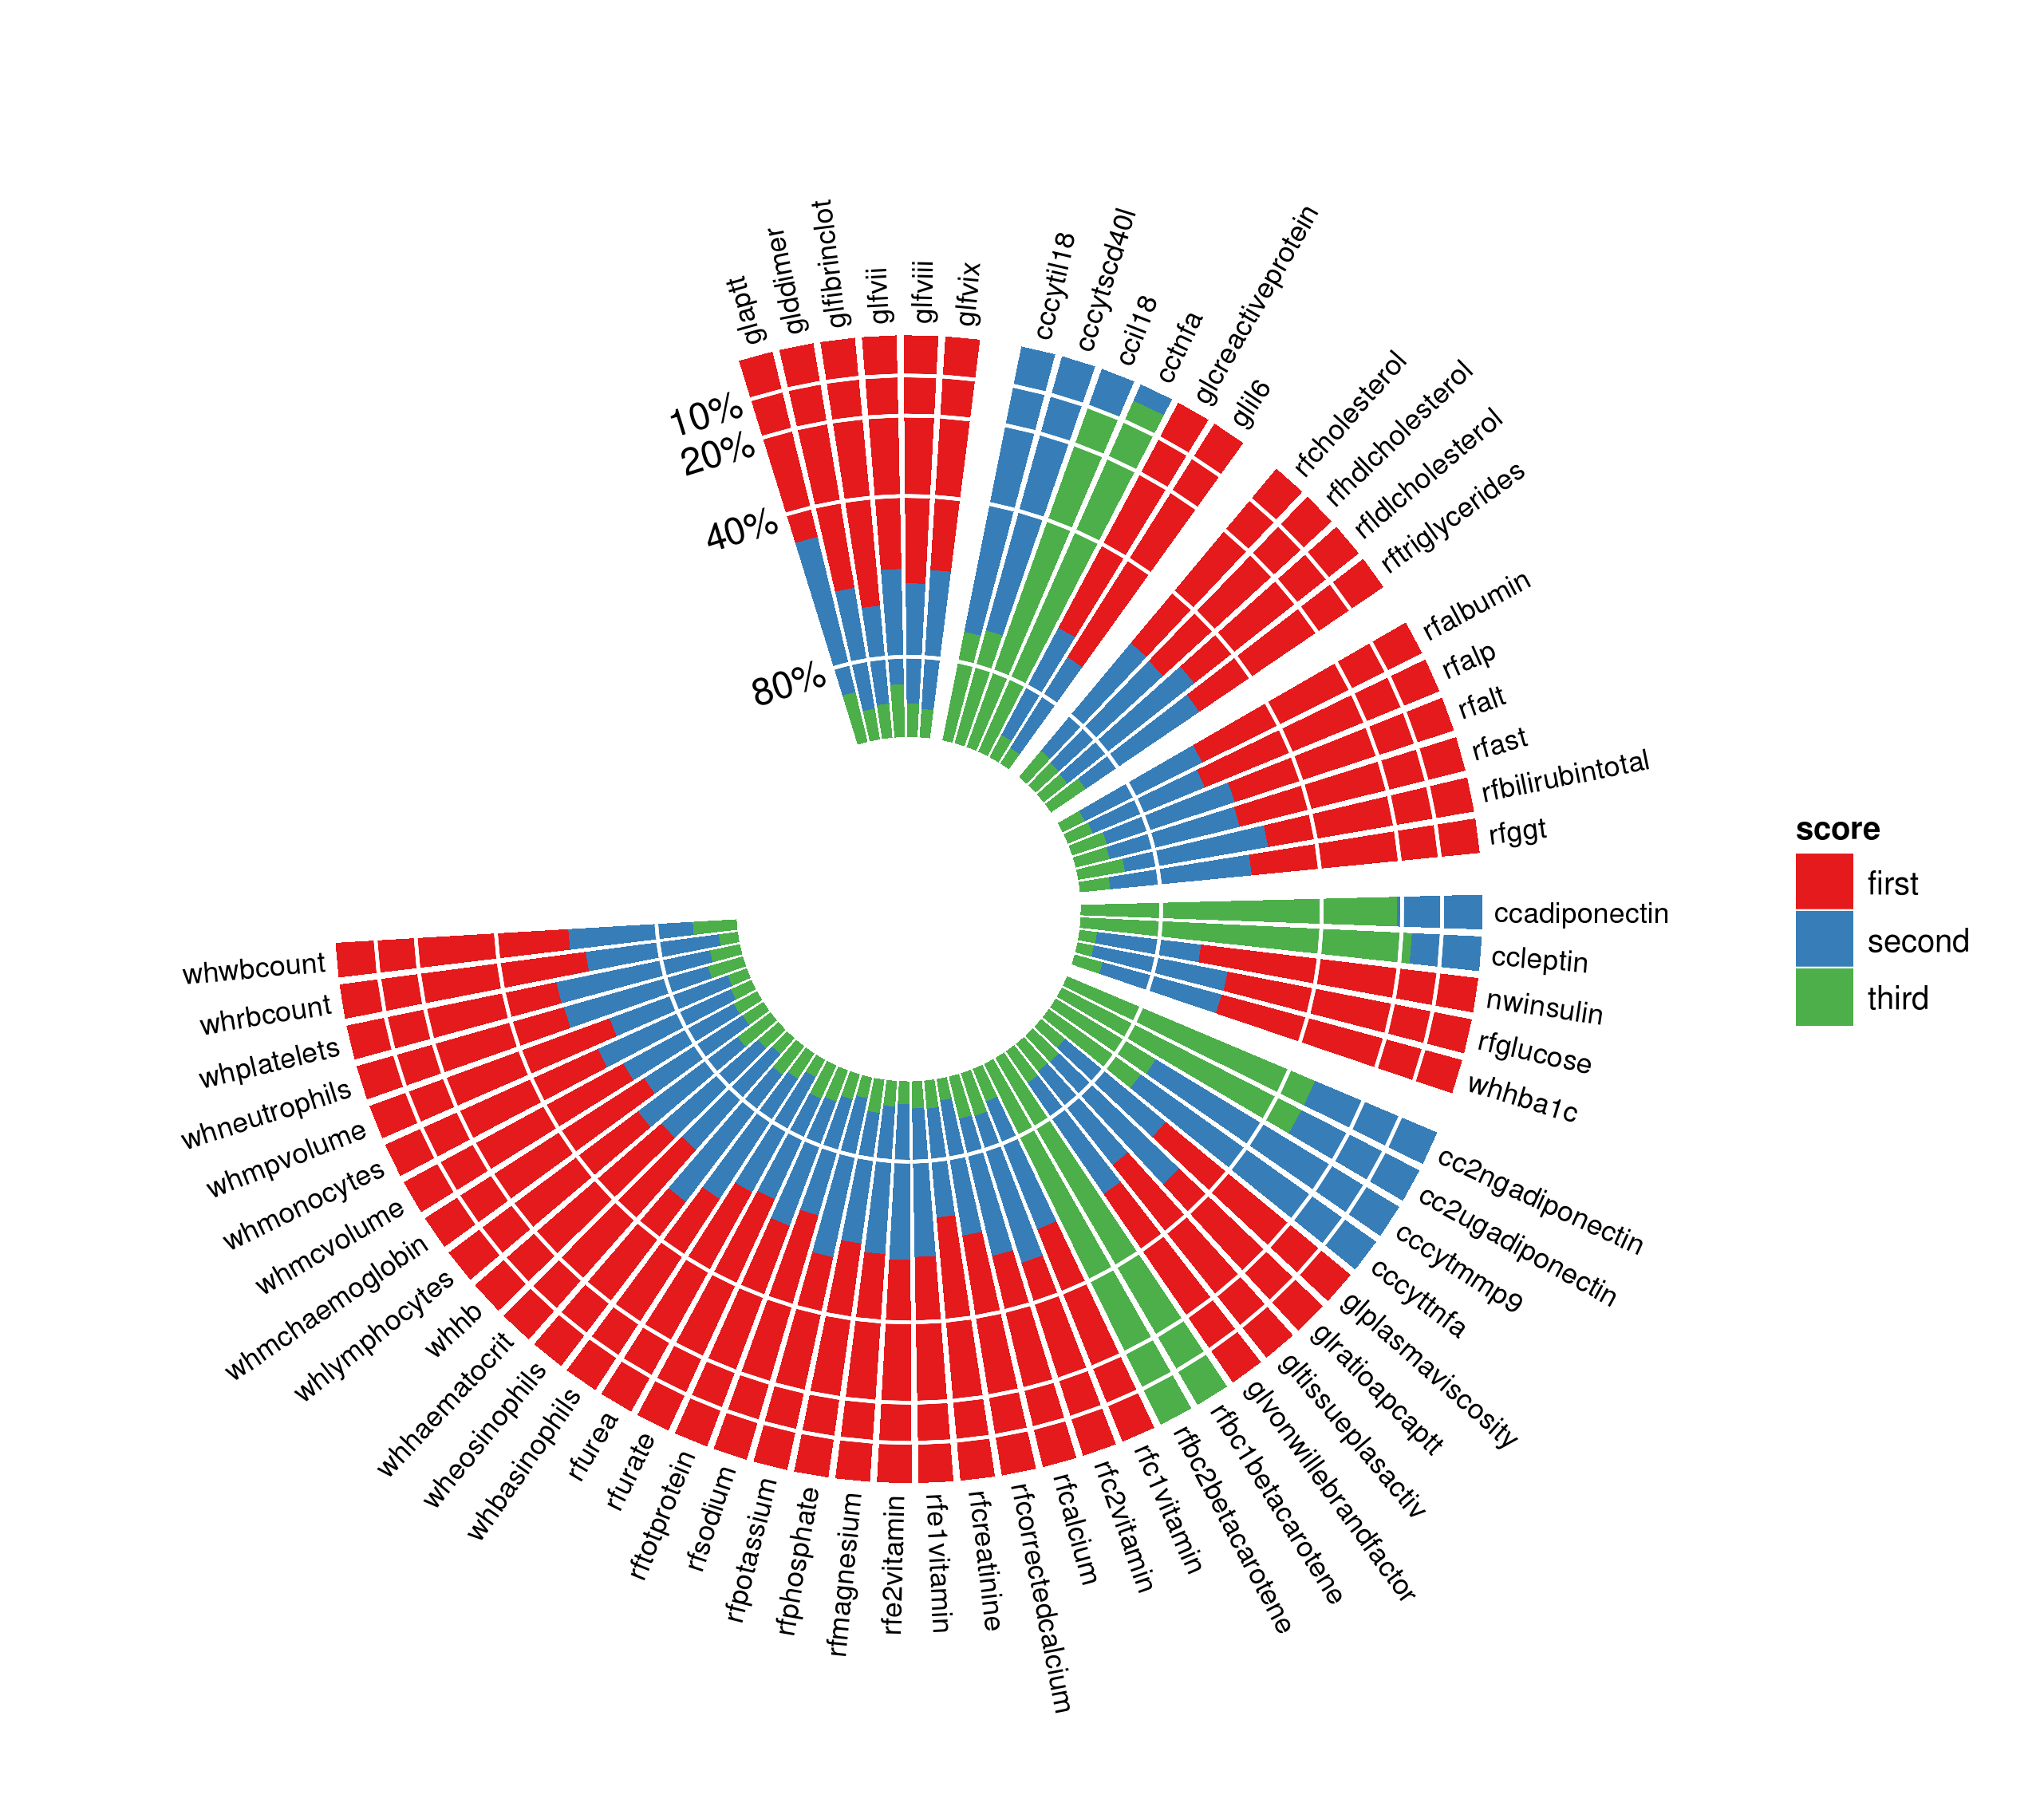
\includegraphics[width=0.9\columnwidth]{Fig/data3.png}
    \caption{Example 3 for Data visualization}
 \end{figure}
%%%%%%%%%%%%%%%%%%%%%%%%%%%%%%%%%%%%%%%%%%%%

%%%%%%%%%%%%%%%%%%%%%%%%%%%%%%%%%%%%%%%%%%%%
 \begin{figure}
    \centering
    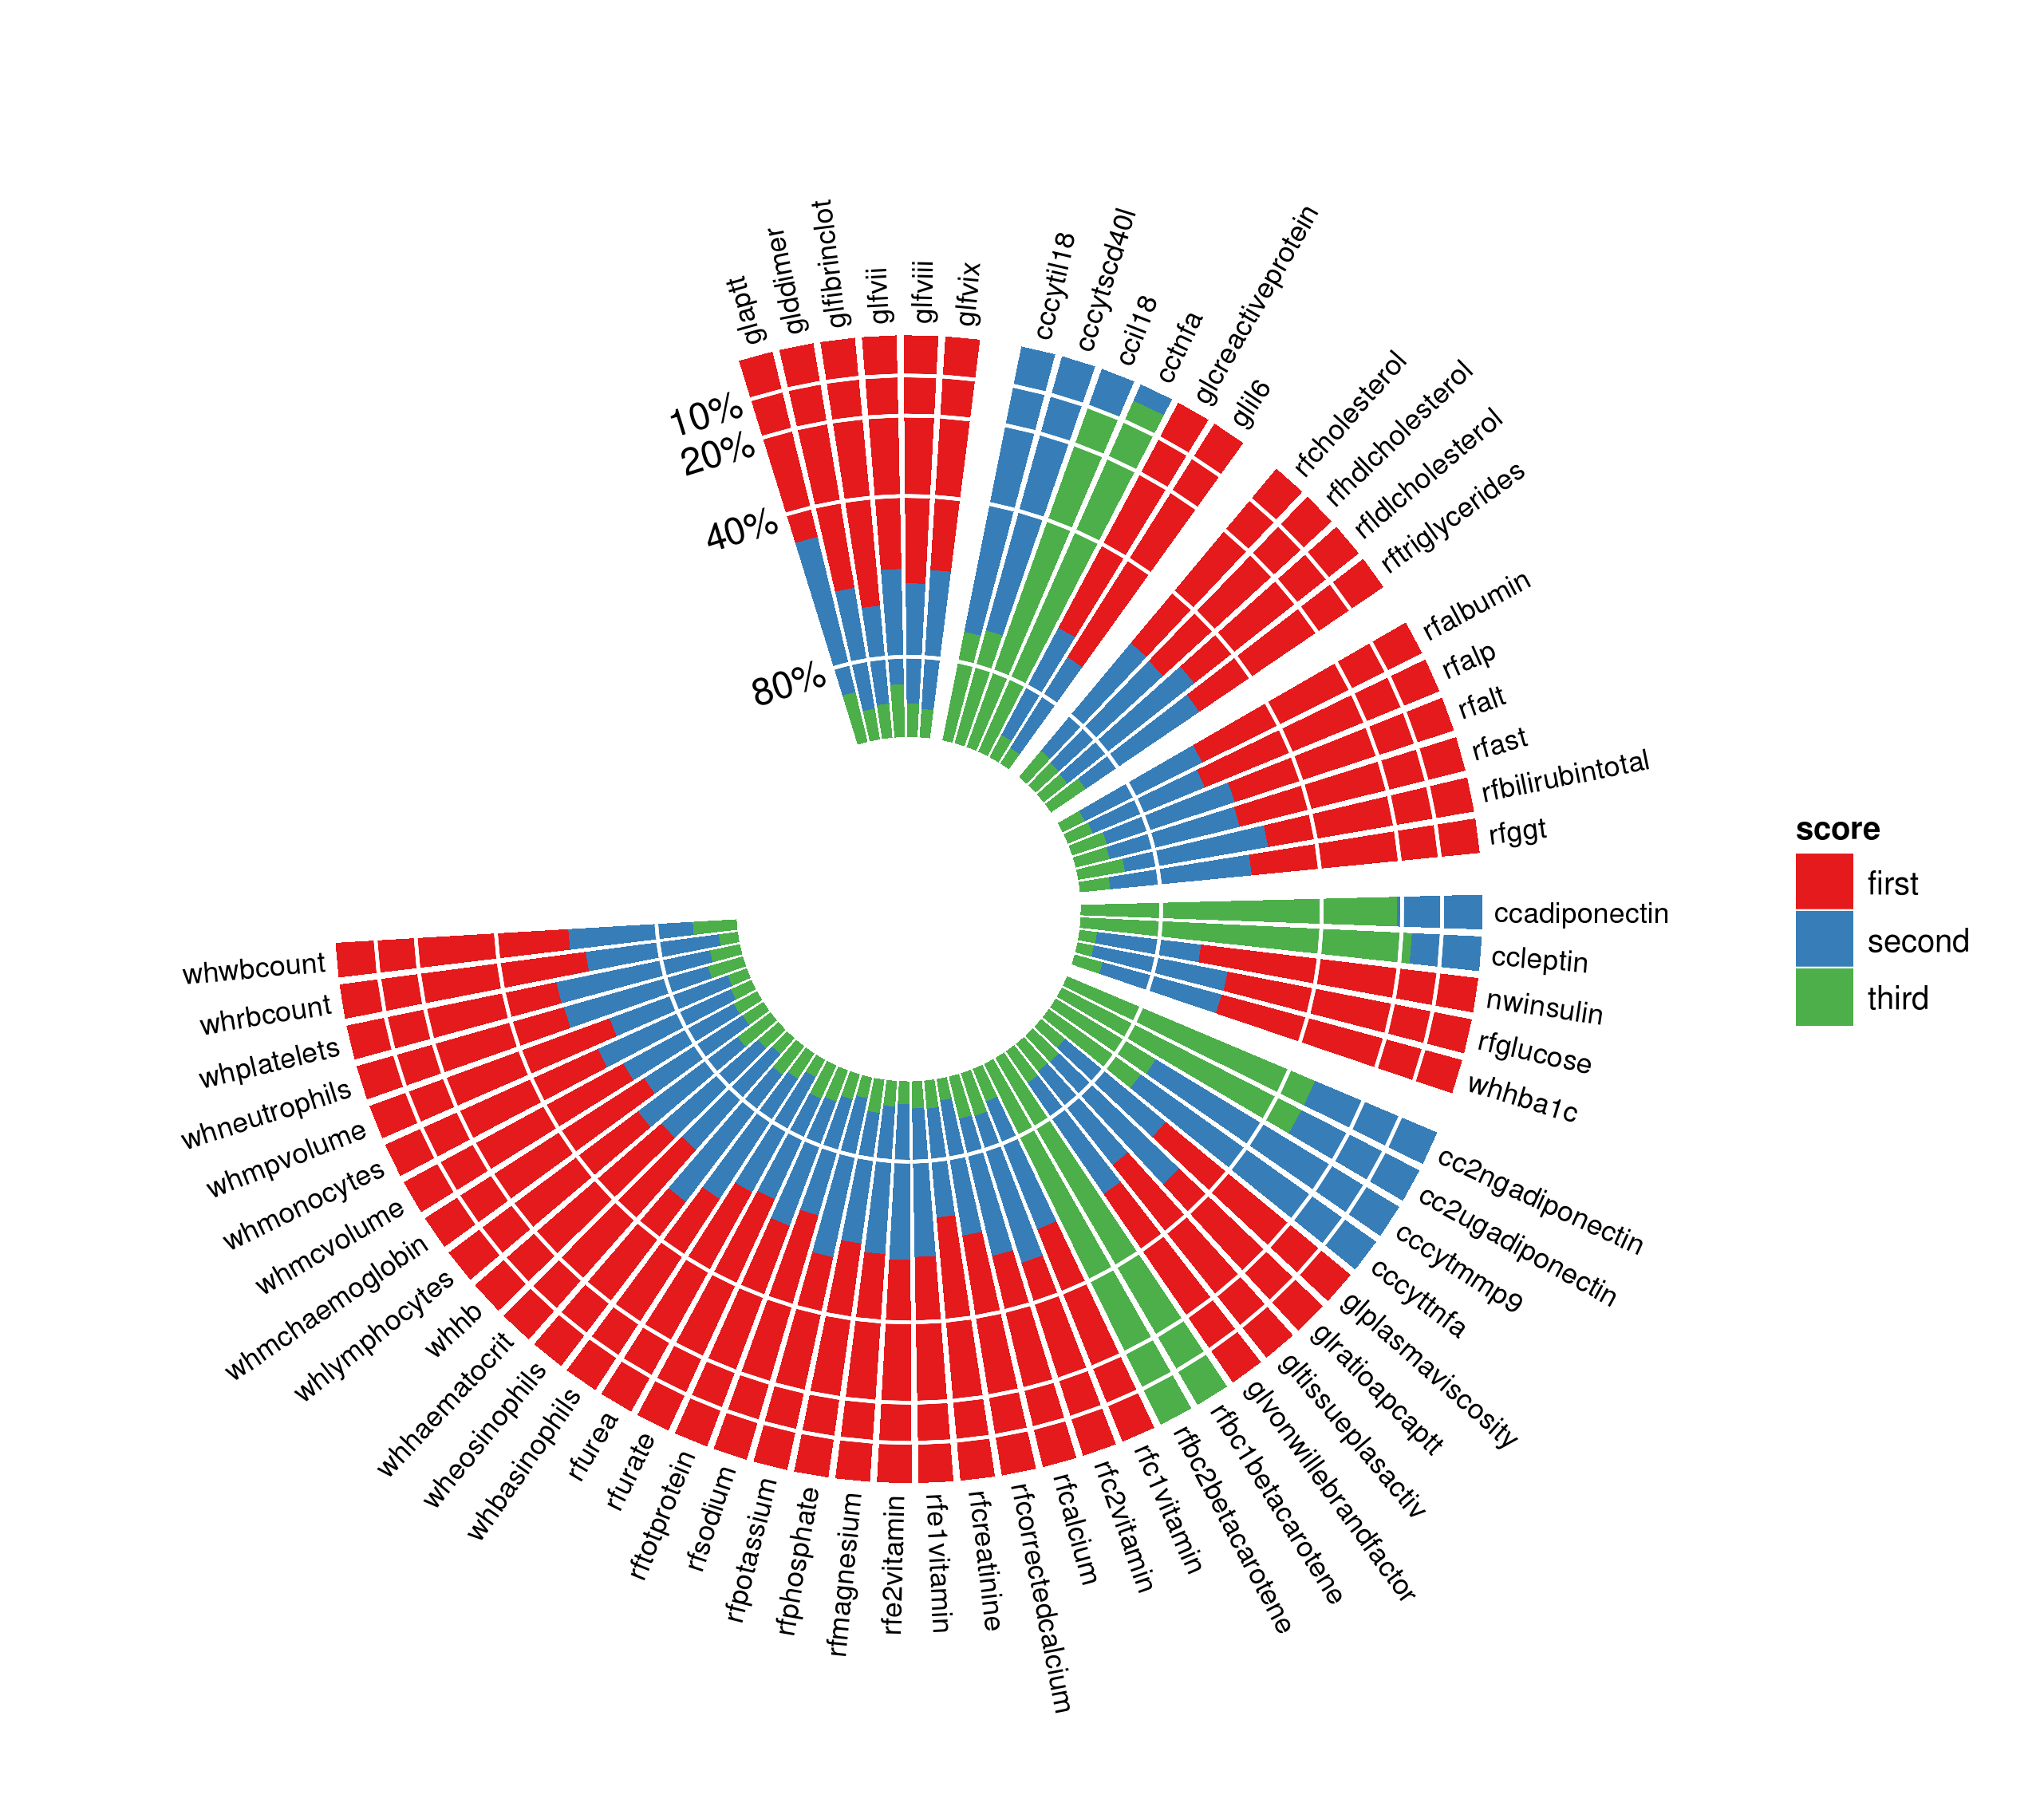
\includegraphics[width=0.9\columnwidth]{Fig/data3.png}
    \caption{Example 4 for Data visualization}
 \end{figure}
%%%%%%%%%%%%%%%%%%%%%%%%%%%%%%%%%%%%%%%%%%%%


\section{Result Analysis}

Please apply what you have learn in class to conduct both theoretical and data analysis of your results.   


\section{Conclusions}

Please state your conclusions here. 

\section*{Acknowledgment}
During this project, I collaborated and discussed with my classmates Si Li, Wu Wang, and Liu Zhao. I also adopted part of contents from Zhihu \cite{Zhihu} to Section II.  



\bibliographystyle{IEEEtran}
\bibliography{Reference}






\end{document}


